\documentclass[11pt]{article}
\usepackage[a4paper,margin=1in]{geometry}
\usepackage{amsmath,amssymb,booktabs,enumitem,mathtools}
\usepackage[T1]{fontenc}
\usepackage[utf8]{inputenc}
\usepackage{lmodern}
\usepackage{graphicx}
\usepackage{hyperref}

\title{Detailed Note on Projection-Based Inference\\for the Rank-1 Matrix Model with $\log_{10}(EC)-\log_{10}(EO)$}
\author{}
\date{\today}

\begin{document}
\maketitle

\section{Purpose}
This note documents the inference procedure used for the ROI-by-band matrix model with predictor
\[
X_i=\log_{10}(EC_i)-\log_{10}(EO_i),
\]
where the matrix rank is fixed at \(r=1\) according to the 5-fold cross-validation analysis. The goal is not to re-select the rank, but to perform valid uncertainty quantification for a prespecified collection of linear functionals of the fitted low-rank coefficient matrix.

The implementation is driven by the scripts
\begin{itemize}[leftmargin=2em]
    \item \texttt{run\_roi10\_matproj\_log\_contrast\_rank1\_ci\_analysis.m},
    \item \texttt{matProj.m},
    \item \texttt{fit\_low\_rank\_trace\_regression.m}.
\end{itemize}

\section{Data and model}
The input file is
\[
\texttt{hbn\_bandpower\_8band\_roi10.mat},
\]
which contains \(N=397\) subjects. For subject \(i\), the analysis uses:
\begin{itemize}[leftmargin=2em]
    \item response \(y_i=\mathrm{age}_i\);
    \item \(10\times 8\) eyes-closed ROI band-power matrix \(EC_i\);
    \item \(10\times 8\) eyes-open ROI band-power matrix \(EO_i\).
\end{itemize}

The matrix regression model is
\[
y_i=\langle X_i,B^\ast\rangle+\varepsilon_i,\qquad \mathrm{rank}(B^\ast)\le 1.
\]
There is no explicit intercept term, so centering is handled inside the inference routine.

\section{Construction of the log-contrast matrix}
Let \(EC_i\) and \(EO_i\) denote the raw ROI power matrices in \(\mu V^2\). Before taking logarithms, the code defines a numerical floor
\[
\text{floor}
=
\max\bigl\{0.5\times \min(\text{positive raw EO/EC entries}),\,10^{-12}\bigr\}.
\]
The transformed matrices are then
\[
\widetilde E_i^{EC}=\log_{10}\!\bigl(\max(EC_i,\text{floor})\bigr),\qquad
\widetilde E_i^{EO}=\log_{10}\!\bigl(\max(EO_i,\text{floor})\bigr),
\]
and the final matrix covariate is
\[
X_i=\widetilde E_i^{EC}-\widetilde E_i^{EO}.
\]
For the current data set, the numerical floor used in this analysis is
\[
2.15735373786\times 10^{-4}.
\]

\section{Inference targets}
The inferential targets are linear functionals of the form
\[
\Delta_T(B^\ast)=\langle T,B^\ast\rangle,
\]
where \(T\) is a user-specified loading matrix. The current analysis evaluates the following prespecified loadings:
\begin{itemize}[leftmargin=2em]
    \item \textbf{single-element loadings}: one loading for each ROI-band entry, yielding \(10\times 8=80\) targets;
    \item \textbf{ROI-slice loadings}: one loading per ROI, with ones across all eight bands, yielding \(10\) targets;
    \item \textbf{band-slice loadings}: one loading per band, with ones across all ten ROIs, yielding \(8\) targets;
    \item \textbf{global loading}: the \(10\times 8\) all-ones matrix, yielding \(1\) target.
\end{itemize}
Every loading is normalized to have unit Frobenius norm before inference.

\section{Cross-fitted inference algorithm}
For a fixed loading \(T\), the function \texttt{matProj(X, y, T, 1)} performs the following steps.

\subsection*{Step 1: random half-splitting}
The \(N=397\) subjects are split into two folds with sizes
\[
n_1=\lfloor N/2\rfloor=198,\qquad n_2=N-n_1=199.
\]
The loading-analysis script resets the random number generator to the common seed
\[
20260321
\]
before every call to \texttt{matProj}, so all loadings are evaluated on the same sample split.

\subsection*{Step 2: fold-specific centering}
Within each half, the matrix predictors and response are centered:
\[
X_i^{(c)}=X_i-\bar X,\qquad y_i^{(c)}=y_i-\bar y.
\]
The stored fold means are later reused to center the opposite evaluation half. Hence the current implementation uses fold-specific centering throughout the initialization, residual construction, and variance calculation.

\subsection*{Step 3: foldwise second moments}
For each training half, the routine computes
\begin{itemize}[leftmargin=2em]
    \item the mode-1 second-moment matrix \(S_1\),
    \item the mode-2 second-moment matrix \(S_2\),
    \item the average squared Frobenius norm \(\overline{\|X\|_F^2}\).
\end{itemize}
These are built from the centered training-half matrices and enter the covariance-weighted projection formulas.

\subsection*{Step 4: low-rank initialization}
On each training half, the initial estimator is obtained by fitting a rank-1 low-rank trace regression to the centered data:
\[
\min_{\mathrm{rank}(B)\le 1}
\frac{1}{2n}\sum_{i=1}^n \bigl(y_i^{(c)}-\langle X_i^{(c)},B\rangle\bigr)^2.
\]
The numerical solver is projected gradient descent with truncated SVD projection:
\begin{enumerate}[leftmargin=2em]
    \item reshape the matrices into a design matrix \(Z\);
    \item compute a step size from the Lipschitz constant \(L=\sigma_{\max}(Z)^2/n\);
    \item take a gradient step;
    \item project back to rank \(1\) by truncated SVD;
    \item stop when the relative coefficient change or the relative objective change falls below \(10^{-7}\), or after \(1000\) iterations.
\end{enumerate}
The output is the rank-1 matrix initializer and its left/right singular vectors.

\subsection*{Step 5: opposite-fold evaluation}
Given a training half and an evaluation half, the evaluation matrices are centered using the \emph{training-half} means. The method then computes:
\begin{itemize}[leftmargin=2em]
    \item the residuals from the training-half initializer;
    \item the empirical score-like matrix \(E_{\mathrm{mean}}\);
    \item the projection direction \(\Phi(T)\) through \texttt{phi\_sigma\_mat};
    \item the projected plug-in term through \texttt{P\_sigma\_mat}.
\end{itemize}
This yields one half-specific estimator of \(\Delta_T(B^\ast)\).

\subsection*{Step 6: cross-fitted point estimator}
The final point estimator averages the two half-specific estimators:
\[
\widehat\Delta_T
=
\frac{\widehat\Delta_T^{(1\leftarrow 2)}+\widehat\Delta_T^{(2\leftarrow 1)}}{2}.
\]
Here the notation indicates that the first superscript half is used for evaluation and the second for training.

\subsection*{Step 7: standard error and confidence interval}
The residuals from both evaluation halves are pooled to estimate \(\sigma^2\). The routine then forms the quadratic variance term
\[
\widehat\Phi
=
\frac{1}{2}\Bigl\{
\Phi_1^\top \bigl[\mathrm{kron}(S_{2,1}^{eval}/\overline{\|X\|_{F,1}^2},\,S_{1,1}^{eval})\bigr]\Phi_1
+
\Phi_2^\top \bigl[\mathrm{kron}(S_{2,2}^{eval}/\overline{\|X\|_{F,2}^2},\,S_{1,2}^{eval})\bigr]\Phi_2
\Bigr\},
\]
and reports
\[
\widehat{\mathrm{sd}}_T=\sqrt{\widehat{\sigma}^2\,\widehat\Phi}.
\]
The nominal \(95\%\) confidence interval is
\[
\widehat\Delta_T \pm 1.96\frac{\widehat{\mathrm{sd}}_T}{\sqrt{N}}.
\]

\section{Current output summary}
The current run evaluates \(99\) loadings in total:
\[
80\ \text{single-element} + 10\ \text{ROI-slice} + 8\ \text{band-slice} + 1\ \text{global}.
\]
The significance summary is:
\begin{itemize}[leftmargin=2em]
    \item \(6/80\) single-element loadings exclude zero;
    \item \(2/10\) ROI-slice loadings exclude zero;
    \item \(1/8\) band-slice loadings exclude zero;
    \item the global loading does not exclude zero.
\end{itemize}

The most important structured results are:
\begin{itemize}[leftmargin=2em]
    \item anterior-midline ROI-slice: \(\hat\delta=0.562\), 95\% CI \([0.169,\,0.956]\);
    \item central-right ROI-slice: \(\hat\delta=-0.529\), 95\% CI \([-0.979,\,-0.080]\);
    \item alpha2 band-slice: \(\hat\delta=0.715\), 95\% CI \([0.243,\,1.187]\);
    \item global loading: \(\hat\delta=0.045\), 95\% CI \([-0.146,\,0.237]\).
\end{itemize}
Thus the inference points to localized structure rather than a uniform matrix-wide shift.

\section{Files generated by the analysis}
The rank-1 matrix inference results are written to:
\begin{itemize}[leftmargin=2em]
    \item \texttt{matproj\_log\_contrast\_rank1\_all\_results.csv},
    \item \texttt{matproj\_log\_contrast\_rank1\_summary.csv},
    \item \texttt{log\_contrast\_rank1\_single\_element\_heatmap.png},
    \item \texttt{log\_contrast\_rank1\_structured\_loadings.png},
    \item \texttt{matproj\_log\_contrast\_rank1\_summary.txt},
    \item \texttt{matproj\_log\_contrast\_rank1\_config.json}.
\end{itemize}

Figure~\ref{fig:structured} reproduces the structured-loading plot written by the script.

\begin{figure}[!ht]
\centering
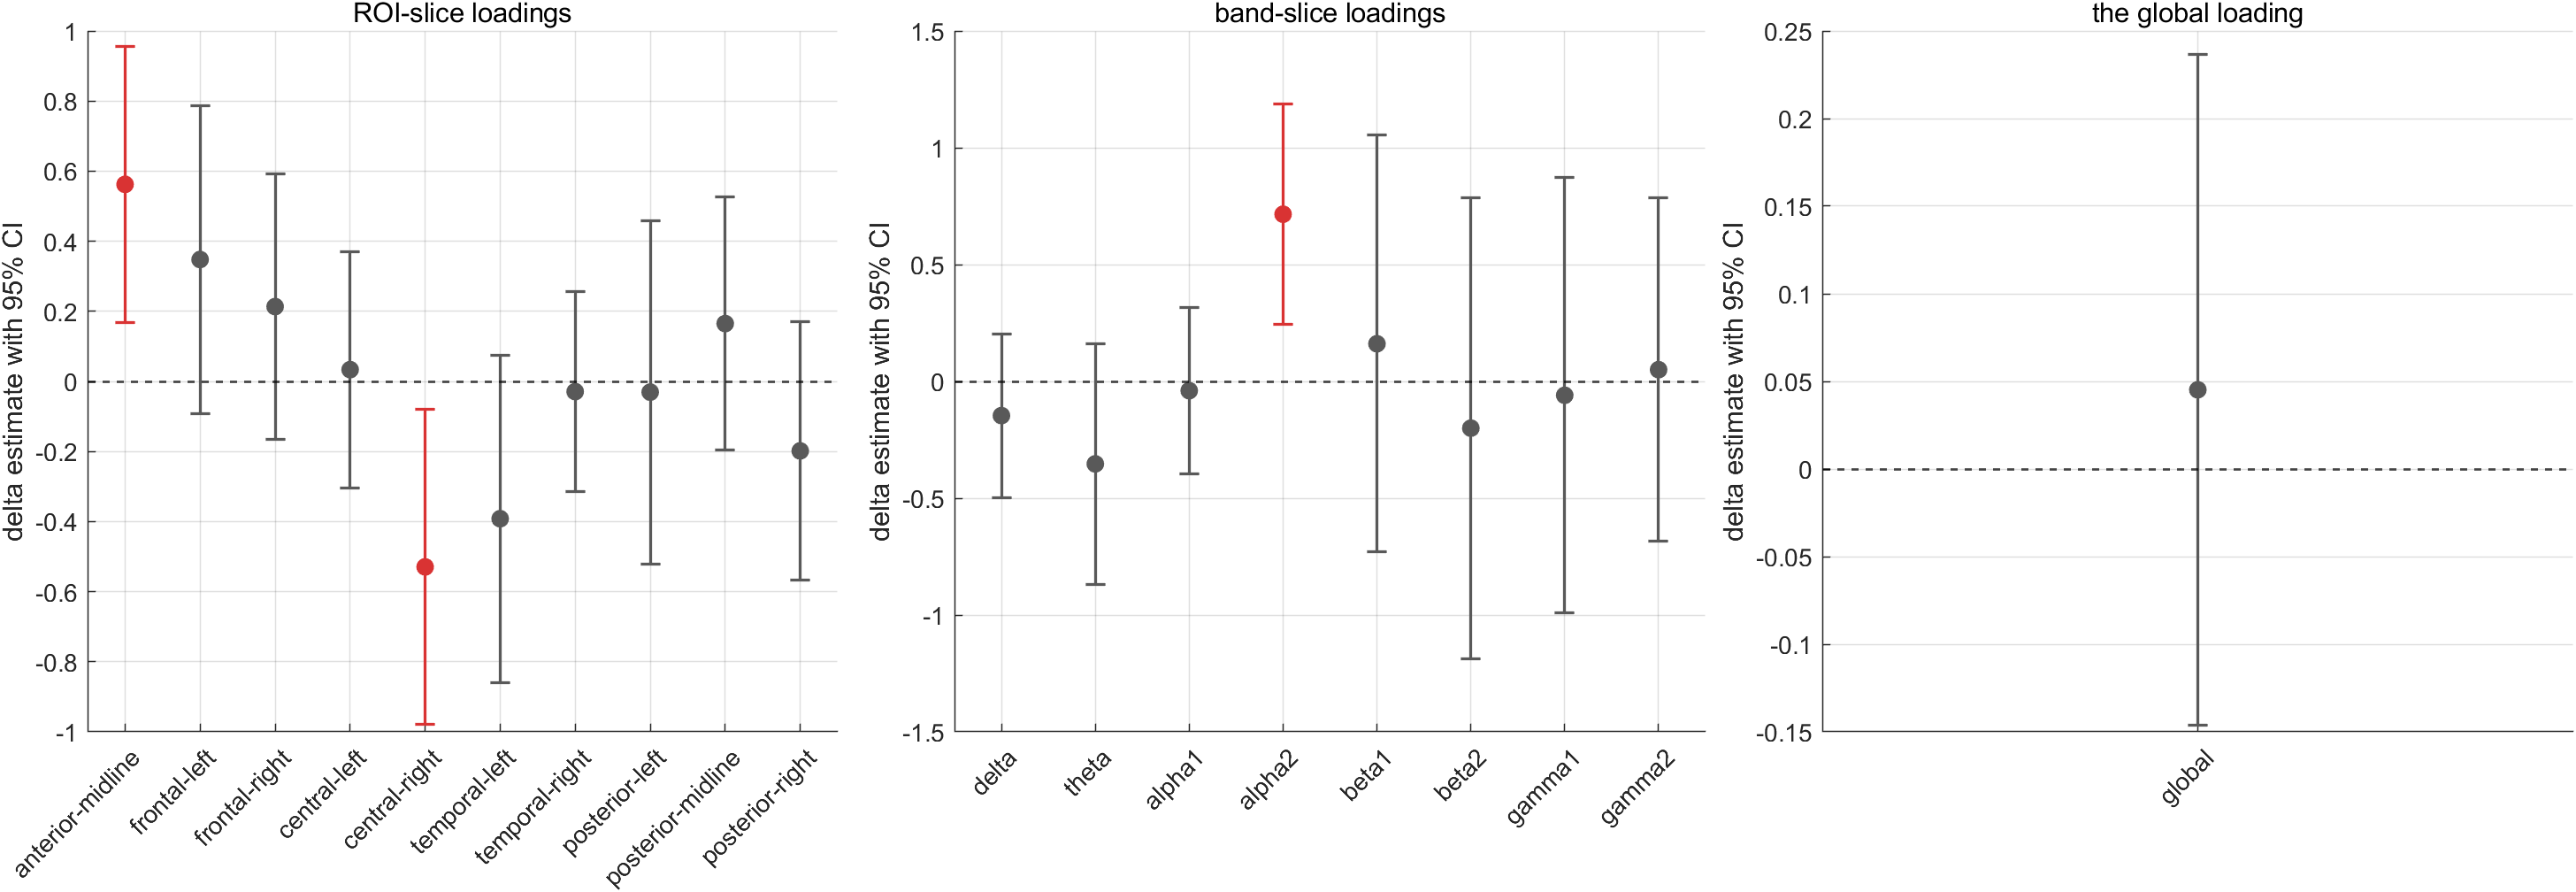
\includegraphics[width=\textwidth]{log_contrast_rank1_structured_loadings.png}
\caption{Projection-based confidence intervals for the ROI-slice, band-slice, and global loadings under the rank-1 log-contrast model.}
\label{fig:structured}
\end{figure}

\section{Interpretation}
From a methodological perspective, this analysis illustrates the role of the proposed projection-based inference framework after rank selection. The rank-1 model is determined by cross-validation, but the scientific conclusions come from the confidence intervals attached to prespecified structured loadings. In the present application, the fitted low-rank log-contrast signal is supported mainly through the anterior-midline and central-right ROI summaries and the alpha2 band summary, whereas the global loading is not distinguishable from zero.

\end{document}
